\documentclass[eclipse]{preziposters}
\usepackage{brackets,importsreferences,amssymb,marvosym,wasysym,pifont,lipsum,symsabim,dingbat,linearb,textcomp}
\usepackage[noend]{algpseudocode}
\title{Graphs \& Optimization}
\suptitle{Doctoral course on}
\author{Willem Van Onsem\\KU Leuven\\Department of Computer Science\\Declarative Languages and Artificial Intelligence}
\logo{../libtex/sedes.pdf}
\disclaimer{This document is published under the \emph{Beer license revision 42} by \emph{Poul-Henning Kamp}.}
\usetikzlibrary{shapes}
\begin{document}

\def\dma{5 mm};
\def\mid{594.5 mm};
\def\dyl{100.0 mm};
\def\dylm{5.0 mm};
\def\dylma{105.0 mm};
\def\dylhma{65.0 mm};
\def\dylqma{150.0 mm};
\def\dyw{1100.0 mm};
\def\dywb{550.0 mm};
\def\dywt{366.7 mm};
\def\dywq{275.0 mm};
\def\dywu{220.0 mm};
\def\dywr{140.0 mm};
\def\dywh{183.3 mm};
\def\dywmbt{458.32 mm};

\definecolor{treebg}{rgb}{0.93,0.93,0.69}

\tikzset{ptgtcov/.style={circle,inner sep=0pt,fill=black,minimum size=1.414mm}}
\tikzset{ptsel/.style={very thick,red}}
\tikzset{ptvir/.style={dashed}}
\tikzset{ptarc/.style={->}}
\tikzset{invisible/.style={opacity=0}}

%formal sink
\definecolor{frml-bg}{RGB}{255,247,220}
\definecolor{frml-fg}{RGB}{224,220,191}
\definecolor{frml-tx}{RGB}{119,119,119}
\newcommand{\frml}[1]{\begin{center}\fcolorbox{frml-fg}{frml-bg}{\parbox{\dimexpr\linewidth-2\fboxsep-2\fboxrule}{\textcolor{frml-tx}{\textit{formal}}\\#1}}\end{center}}
\newcommand{\fcop}[3][+]{\ifthenelse{\equal{#1}{+}}{\renewcommand{\fcopm}{maximize}}{\renewcommand{\fcopm}{minimize}}\[\begin{array}{lll}\mbox{\fcopm{}}&\multicolumn{2}{l}{#2,}\\\mbox{subject to}&#3\end{array}\]}
\newcommand{\fsat}[1]{\[\begin{array}{lll}\mbox{satisfy}&#1\end{array}\]}

\defgroup[\dma][0][-0.5*\dylma-\dylqma][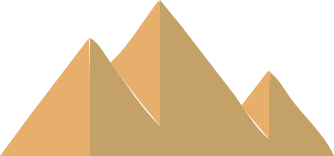
\includegraphics{pyramid.pdf}]{\dyw-\dywt}{\dylqma}{Basics}{orange}{graph}
\defgroup[\dma][2*\dywt][-0.5*\dylma-\dylqma][
\includegraphics{family.pdf}]{\dywt}{\dylqma}{Graph families}{purple}{grfa}
\defgroup[\dma][0][-0.5*\dylma-2*\dylqma][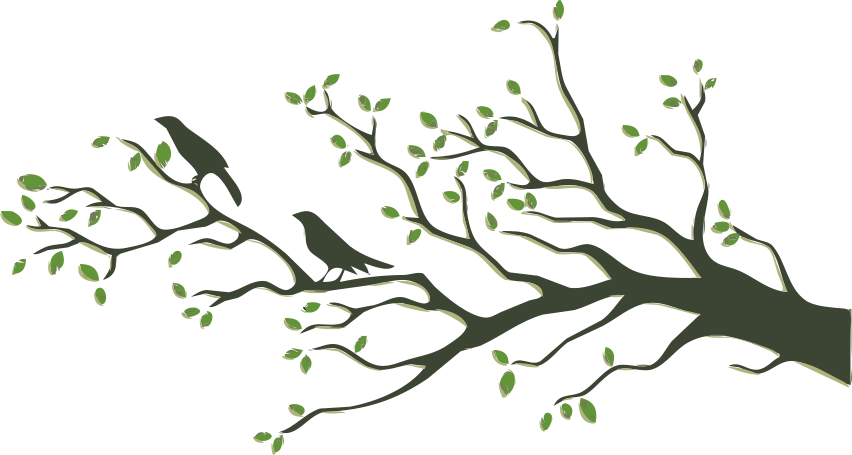
\includegraphics{tree.pdf}]{\dywb}{\dylqma}{Trees}{treebg}{tree}
\defgroup[\dma][\dywb][-0.5*\dylma-2*\dylqma][
\includegraphics{walk.pdf}]{\dywb}{\dylqma}{Walks and Reachability}{yellow}{move}
\defgroup[\dma][0][-0.5*\dylma-3*\dylqma][\includegraphics{barcode.pdf}]{\dyw-\dywu-\dywb}{\dylqma}{Codes \& sequences}{blue}{cseq}
\defgroup[\dma][\dyw-\dywu-\dywb][-0.5*\dylma-3*\dylqma][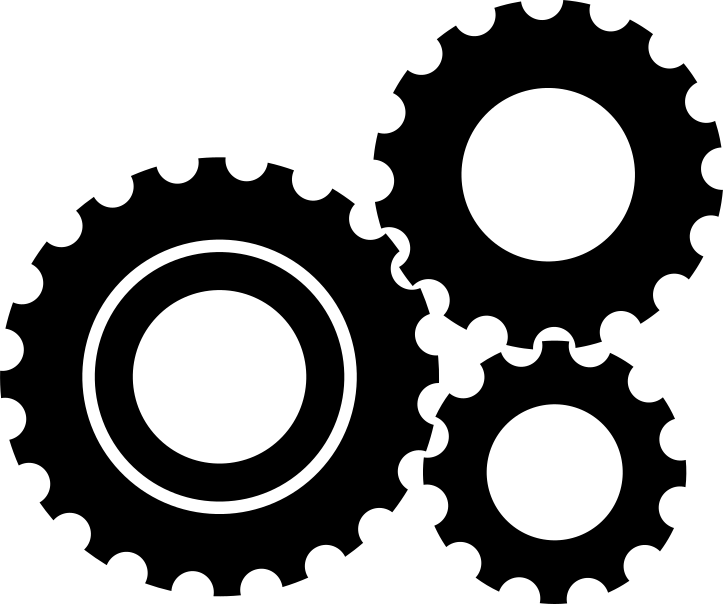
\includegraphics{gear.pdf}]{\dywb+\dywu}{\dylqma}{Optimization problems \& greedy algorithms}{green}{cop}
\defgroup[\dma][0][-0.5*\dylma-4*\dylqma][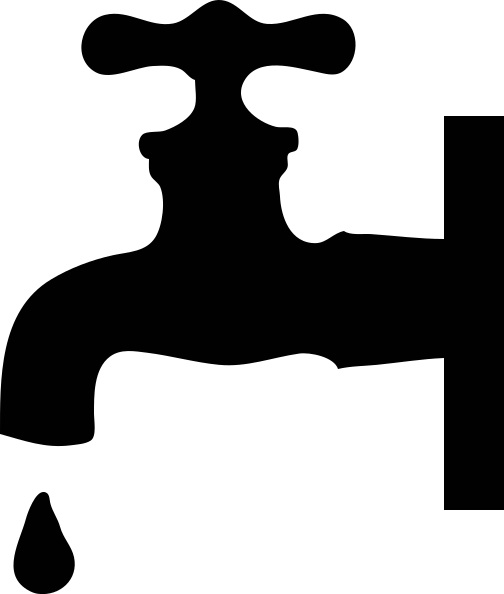
\includegraphics{flow.pdf}]{\dywmbt-0.5*\dywr}{\dylqma}{Maximum flow}{purple}{maflw}
\defgroup[\dma][\dywmbt-0.5*\dywr][-0.5*\dylma-4*\dylqma][
\includegraphics{palette.pdf}]{\dyw-\dywmbt-0.5*\dywr}{\dylqma}{Graph coloring}{red}{grcl}

%Legend
\defgroup[\dma][\dyw-\dywr][-0.5*\dylma-4*\dylqma][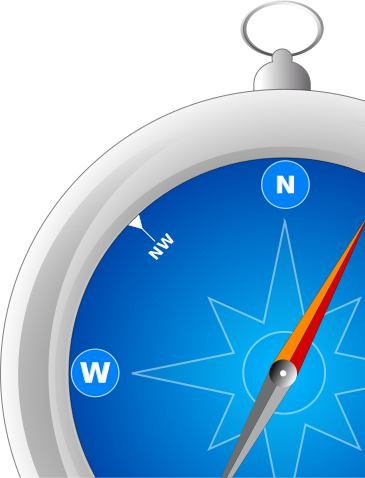
\includegraphics{compass.pdf}]{\dywr}{\dylqma}{Legend}{backg}{legen}
\subgrouptable[6 cm/ver/Vertices,6 cm/arc/{Edges/Arcs}]{legen}

\arcoverview[(0.25,-1)][5 cm]{legen-arc}{{very thick,black!80!white}//{Related concepts},{very thick,black!80!white,->}//{Reference},{very thick,open triangle 60-,black!80!white}//{Second concept implies first}}

%Definitions
\boxfile{definitions.tex}

%Theorems
\def\pztbtc{red}
\boxfile{theorems.tex}

%Algorithms
\def\pztbtc{blue}
\boxfile{algorithms.tex}

%Applications
\def\pztbtc{orange}
\boxfile{app.tex}

%Images
\tikzminibox[(graph)][grphvw][16.75][1]{grph}
\tikzminibox[(grcl)][grclvw][20.5][10.75]{grcl}

%Relations
\confile[very thick,black!80!white][sloped,above,midway,black]{rels.tex}
%Subset relations
\confile[very thick,open triangle 60-,black!80!white][sloped,above,midway,black]{subs.tex}
%Subset relations
\confile[very thick,black!80!white,->][sloped,above,midway,black]{refe.tex}

\groupbox{(CCgraycod) (CChypergr)}{Bitwise graphs}
\groupbox{(CCcncwl) (CCsubwl)}{Walk operations}
\groupbox{(CCeulert) (CCceuler) (CCposttour) (CChamilcyc) (CCctreuler)}{Special walks}
\groupbox{(CCreach) (CCconn) (CCwkconn) (CCedgcut) (CCvercut) (CCcpn)}{Reachability and components}
\groupbox{(CCprnttree) (CCdscasctree)}{Rooted tree vertex relations}
\groupbox{(CCstree) (CCfronted) (CCtreegrow)}{Tree growing}
\groupbox{(CCmarytree) (CCordtree) (CCbintree) (CCtreecv)}{Tree variants}
\groupbox{(CCgruni) (CCgrjoin) (CCvdsg) (CCedsg) (CCsbgiv) (CCsbgie) (CClinegr)}{Graph operations}
\groupbox{(CCsubgr) (CCcliq)}{Graph substructures}
\groupbox{(CCince) (CCadjv) (CCadje) (CCongbrh) (CCcngbrh)}{Relations between vertices and edges}
\groupbox{(CCslfl) (CCdegv) (CCeulerthm) (CCmule)}{Edge types and degrees}
\groupbox{(CCindepset) (CCmatching)}{Independence and matchings}
\groupbox{(CCherdss) (CCgreed)}{Maximum-weight problem}
\groupbox{(CCproj) (CCaoan) (CCcpm)}{Project scheduling}
\groupbox{(CChungarian) (CCsdr) (CCassg)}{Representation allocation}
\groupbox{(CCloccol) (CClocextcol)}{Robust coloring}
\groupbox{(CCgrcl1) (CCgrcl2) (CCgrcl3)}{Graph coloring problem variants}

\end{document}